% rubber: setlist arguments -shell-escape
% Important: The shell-escape flag is required for the Minted package.
% Please compile this document with 'pdflatex -shell-escape main.tex'.
% If you are using another IDE, you may be able to specify this in the
% options or to provide an option like '% !TEX option = -shell-escape'
% in this file, depending on your builder. See the README.md for more.

% Don't put any content in here.
% Don't even include content files by using \input or \inlcude.
% Put your content into components/text.tex or include it there using \input.
% You probably want to modify the following files:
%   components/info.tex             contains the author, title etc.
%   components/settings.tex         contains the packages and settings.
%   components/commands.tex         contains helpful custom commands.
%   components/glossary.tex         contains an explanation of the used terms.
%   components/acknowledgements.tex contains the acknowledgements.
%   components/quote.tex            contains a quote.
%   components/abstract.tex         contains the abstract of the document.
%   components/text.tex             includes the actual content of the document.
%   components/outline.tex          contains the outline.
%   components/preface.tex          contains the preface.
%   chapters/                       contains the main text.
%   bibliography/literature.bib     contains the BibTeX entries.
%   images/                         contains all your content-related images.
%
% You probably don't need to change anything in the following files:
%   components/cover.tex            formats the front cover of the document.
%   components/titlepage.tex        formats the title page of the document.
%   components/disclaimer.tex       formats the disclaimer page.
%   styles/                         contains style elements (e.g. logos).
%   main.tex                        contains the top-level code structure.
%   README.md                       contains information about this template.

\documentclass[12pt,
              letter,
              index=totoc,
              headsepline,
              footsepline,
              BCOR=12mm,
              DIV=13,
              parskip=half,
              enabledeprecatedfontcommands]{scrbook}

% KOMA scrbook options:
%  index=totoc: include an entry for the index in the table of contents.
%  headsepline: use horizontal line under heading.
%  footsepline: use horizontal line above footer.
%  BCOR: binding correction (e.g.: BCOR=12mm)
%  DIV: Number of sheet sections (used for layout) (e.g.: DIV=13)

% !TEX root = ../main.tex
% Set here the title, authors and other stuff to be used for the cover
% This file is used by MAIN.TEX

% set title, authors and stuff for the cover
\def\university{Universidad de los Andes}
\def\universityLogo{styles/tum_logo}
\def\program{Master of Systems and Computing Engineering}
\def\programLogo{styles/cse_logo}
\def\doctype{Master's Thesis}

\def\title{Bounded generics over constants in Rust}
\def\author{Christian Nicanor Poveda Ruiz}
\def\examinerOne{Silvia Takahashi}
\def\examinerTwo{Oliver Scherer}
\def\assistantAdvisor{Nicolás Cardozo Alvarez}
\def\date{2019-05-24}

\def\keywords{{keyword1}, {keyword2}, {keyword3}}

% The following are used for the PDF metadata, by default the same as above.
\def\metaTitle{\title}
\def\metaAuthor{\author}
\def\metaSubject{\doctype\ -\ \university}
\def\metaKeywords{\keywords}

% text to appear in the footer
\def\footertext{}


% !TEX root = ../main.tex
% Included by MAIN.TEX

%--------------------------------------------------
% Fonts and page setup
%--------------------------------------------------

% Default font
\usepackage{palatino}
\usepackage{sourcecodepro}
\usepackage[T1]{fontenc}
% Enable special PostScript fonts (optional)
% \usepackage{pifont}

% Manipulate the footer
\usepackage{scrlayer-scrpage}
\usepackage{scrhack}
\pagestyle{scrheadings}
\ifoot[\footertext]{\footertext} % \footertext set in INFO.TEX

% Set the font for the section headings
\renewcommand{\sectfont}{\normalfont \bfseries}

% Conditional commands in LaTeX documents, used for the \clearemptydoublepage.
\usepackage{ifthen}

% Typeset text in multiple columns (optional)
% \usepackage{multicol}

% Rotation tools, including rotated full-page floats (optional)
\usepackage{rotating}


%--------------------------------------------------
% Document structure
%--------------------------------------------------

% Pro­duce hy­per­text links in the doc­u­ment (recommended)
\usepackage{hyperref}

% Create glossaries and lists of acronyms
% depending on how many packages were shipped with your TeX distribution,
% you might need to install xindy. On Linux: sudo apt install xindy
\usepackage[toc, xindy]{glossaries}

% Standard LaTeX package for creating indexes
\usepackage{makeidx}


%--------------------------------------------------
% Bibliography
%--------------------------------------------------

% Set the bibliography style (default: plain)
\bibliographystyle{plainnat}

% Special biblography package (nice to have)
\usepackage[numbers]{natbib}

%--------------------------------------------------
% Graphics and floats
%--------------------------------------------------

% Enhanced support for graphics (recommended)
\usepackage{graphicx}
% Path to the figures directory (default: {figures/})
% Multiple entries are allowed, e.g. {{figures1/}{figures2/}}.
\graphicspath{{figures/}}

% Improved interface for floating objects (optional)
\usepackage{float}

% To use the subfigures (optional)
\usepackage{subcaption}


%--------------------------------------------------
% Mathematics
%--------------------------------------------------

% AMS mathematical facilities for LaTeX (recommended)
\usepackage{amsmath}

% TeX fonts from the American Mathematical Society (recommended)
\usepackage{amsfonts}

% Some extra math symbols (optional)
\usepackage{amssymb}

% Extended maths fonts for LaTeX (optional)
% \usepackage{yhmath}

% Provide math delimiters whose size can be computed automatically (optional)
% \usepackage{commath}


%--------------------------------------------------
% Source code and algorithms
%--------------------------------------------------

% Source code typesetting
% \usepackage{listings} % (optional - alternative)
\usepackage[newfloat]{minted} % (recommended)
% Set global Minted options
\setminted{linenos, autogobble, frame=lines, framesep=2mm}
\usemintedstyle{perldoc}

% Inline C++ (optional)
\newcommand{\inrust}[1]{\mintinline{rust}{#1}}
\newenvironment{code}{\captionsetup{type=listing}}{}
\SetupFloatingEnvironment{listing}{name=Listing}

% Typeset algorithms - pseudocode (optional)
% \usepackage{algorithmicx}
% \usepackage{algpseudocode}
% Normal arrow comments
% \algrenewcommand{\algorithmiccomment}[1]{\hfill$\rightarrow$ #1}


%--------------------------------------------------
% Tables
%--------------------------------------------------

% Tables (optional)
\usepackage{tabu}

% Add color to LaTeX tables (optional)
% \usepackage{colortbl}

% Create tabular cells spanning multiple rows (optional)
% \usepackage{multirow}


%--------------------------------------------------
% Color
%--------------------------------------------------

% Use colors
\usepackage[dvipsnames]{xcolor}

% You may find all the pre-defined colors in
% https://en.wikibooks.org/wiki/LaTeX/Colors#Predefined_colors

% Custom colors
\definecolor{Pantone300C}{HTML}{0065BD} % TUM primary blue
\definecolor{Pantone301}{HTML}{005293}  % TUM secondary light blue
\definecolor{Pantone540}{HTML}{003359}  % TUM secondary dark blue
\definecolor{DarkGray}{HTML}{333333}    % TUM secondary dark gray
\definecolor{MediumGray}{HTML}{808080}  % TUM secondary medium gray
\definecolor{LightGray}{HTML}{CCCCC6}   % TUM secondary light gray
\definecolor{Pantone7527}{HTML}{DAD7CB} % TUM accent gray
\definecolor{Pantone158}{HTML}{E37222}  % TUM accent orange
\definecolor{Pantone383}{HTML}{A2AD00}  % TUM accent green
\definecolor{Pantone283}{HTML}{98C6EA}  % TUM accent very light blue
\definecolor{Pantone542}{HTML}{64A0C8}  % TUM accent light blue

% Color for the hyperlinks (e.g. table of contents)
\def\colorLinks{Pantone300C}
% Color for the web links
\def\colorUrl{Pantone542}
% Color for the citations
\def\colorCitations{Pantone158}

%--------------------------------------------------
% PDF output
%--------------------------------------------------

% Adjust the color of the links
\hypersetup{
  linkcolor=\colorLinks,%
  urlcolor=\colorUrl,%
  citecolor=\colorCitations
}

% Disable the coloring of the links when printing.
% Requires a compatible PDF reader.
\usepackage[ocgcolorlinks]{ocgx2}[2017/03/30]

% PDF Metadata
\hypersetup{
  pdftitle={\metaTitle},%
  pdfauthor={\metaAuthor},%
  pdfkeywords={\metaKeywords},%
  pdfsubject={\metaSubject}
}

% Create XMP Metadata (uses the values from hyperref)
\usepackage{hyperxmp}

% Make thumbnails (optional)
% \usepackage{thumbpdf}


%--------------------------------------------------
% Other settings
%--------------------------------------------------

% Define commands that appear not to eat spaces (optional)
\usepackage{xspace}

% Fancyref
\usepackage[plain]{fancyref}

\usepackage{makecell}


% !TEX root = ../main.tex
% Included by MAIN.TEX
% Please include your own cool commands here.
% Be only sure to comment it sufficiently so others can use it.

%-------------------------------------------------------------
%                      Own Commands
%-------------------------------------------------------------


%-------------------------------------------------------------
% math stuff -------------------------------------------------

% nice R, N, C
\newcommand{\nat}{\mathbb{N}}
\newcommand{\real}{\mathbb{R}}
\newcommand{\compl}{\mathbb{C}}

% norm
%\newcommand{\norm}[1]{\left\| #1 \right\|}

% un demi
\newcommand{\half}{\frac{1}{2}}

% parantheses
\newcommand{\parenth}[1]{ \left( #1 \right) }
\newcommand{\bracket}[1]{ \left[ #1 \right] }
\newcommand{\accolade}[1]{ \left\{ #1 \right\} }
%\newcommand{\angle}[1]{ \left\langle  #1 \right\rangle }

% partial derivative: %#1 function, #2 which variable
% simple / single line version
\newcommand{\pardevS}[2]{ \delta_{#1} f(#2) }

% fraction version
\newcommand{\pardevF}[2]{ \frac{\partial #1}{\partial #2} }

% render vectors: 3 and 4 dimensional
\newcommand{\veciii}[3]{\left[ \begin{array}[h]{c} #1 \\ #2 \\ #3	\end{array} \right]}
\newcommand{\veciv}[4]{\left[ \begin{array}[h]{c} #1 \\ #2 \\ #3 \\ #4	\end{array} \right]}

% render matrices: 3  dimensional (arguments in row first order)
\newcommand{\matiii}[9]{\left[ \begin{array}[h]{ccc} #1 & #2 & #3 \\ #4 & #5 & #6 \\ #7 & #8 & #9	\end{array} \right]}


%-------------------------------------------------------------
%-------------------------------------------------------------


%-------------------------------------------------------------
% some abreviations ------------------------------------------
\newcommand{\Reg}{$^{\textregistered}$}
\newcommand{\reg}{$^{\textregistered}$ }
\newcommand{\Tm}{\texttrademark}
\newcommand{\tm}{\texttrademark~}
\newcommand {\bsl} {$\backslash$}

%-------------------------------------------------------------
%-------------------------------------------------------------


%-------------------------------------------------------------
% formating --------------------------------------------------

% Theorem & Co environments and counters
\newtheorem{theorem}{Theorem}[chapter]
\newtheorem{lemma}[theorem]{Lemma}
\newtheorem{corollary}[theorem]{Corollary}
\newtheorem{remark}[theorem]{Remark}
\newtheorem{definition}[theorem]{Definition}
\newtheorem{equat}[theorem]{Equation}
\newtheorem{example}[theorem]{Example}
%\newtheorem{algorithm}[theorem]{Algorithm}

% inserting figures
\newcommand{\insertfigure}[4]{ % Filename, Caption, Label, Width percent of textwidth
	\begin{figure}[htbp]
		\begin{center}
			\includegraphics[width=#4\textwidth]{#1}
		\end{center}
		\vspace{-0.4cm}
		\caption{#2}
		\label{#3}
	\end{figure}
}

% referecing figures

\newcommand{\refFigure}[1]{ %label
	figure \ref{#1}
}
\newcommand{\refChapter}[1]{ %label
	chapter \ref{#1}
}

\newcommand{\refSection}[1]{ %label
	section \ref{#1}
}

\newcommand{\refParagraph}[1]{ %label
	paragraph \ref{#1}
}

\newcommand{\refEquation}[1]{ %label
	equation \ref{#1}
}

\newcommand{\refTable}[1]{ %label
	table \ref{#1}
}

\newcommand{\rigidTransform}[2]
{
	${}^{#2}\!\mathbf{H}_{#1}$
}

% comment that appears on the border - very practical !!!
\newcommand{\comment}[1]{\marginpar{\raggedright \noindent \footnotesize {\textsl{#1}} }}

% page clearing
\newcommand{\clearemptydoublepage}{%
  \ifthenelse{\boolean{@twoside}}{\newpage{\pagestyle{empty}\cleardoublepage}}%
  {\clearpage}}

%-------------------------------------------------------------
%-------------------------------------------------------------

\newcommand{\etAl}{\emph{et al.}\mbox{ }}

% Fancyref
\newcommand*{\fancyreflistingprefix}{lst}
\newcommand*{\fancyrefsubsectionprefix}{subsec}
\frefformat{plain}{\fancyreflistingprefix}{listing\fancyrefdefaultspacing#1}
\Frefformat{plain}{\fancyreflistingprefix}{Listing\fancyrefdefaultspacing#1}
\frefformat{plain}{\fancyrefsubsectionprefix}{subsection\fancyrefdefaultspacing#1}
\Frefformat{plain}{\fancyrefsubsectionprefix}{Subsection\fancyrefdefaultspacing#1}


% !TEX root = ../main.tex
\newglossaryentry{computer}
{
  name=computer,
  description={is a programmable machine that receives input,
               stores and manipulates data, and provides
               output in a useful format}
}

\newglossaryentry{poc}
{
  name={proof of concept},
  description={}
  }
\newglossaryentry{ui}
{
  name={user interface},
  description={}
  }
\newglossaryentry{ai}
{
  name={arithmetic intensity},
  description={a measure of floating-point operations (FLOPs)
              \hyphenation{per-formed} performed by a \hyphenation{gi-ven} given code or code section relative
              to the amount of memory accesses (Bytes) that are required
               to support those operations\cite{AI}}
  }

\newglossaryentry{speed-up}
{
  name={speed-up},
  description={the factor of temporal acceleration a program
  exhibits when additional computational resources are dedicated to it's execution.}
}

\newglossaryentry{directive pragmas}
{
  name={directive pragma},
  description={a computer programming language construct that specifies how a compiler
  should process input data} % sourced from wikipedia
}


\newglossaryentry{rc}{%SOURCE: wikipedia
name={race condition},
description={A race condition or race hazard is the behavior of an electronic,
 software, or other system where the output is dependent on the sequence or
 timing of other uncontrollable events. It becomes a bug when events do not
 happen in the order the programmer intended. The term originates with the idea
 of two signals racing each other to influence the output first.}
}
\newglossaryentry{dd}{
name={data dependencies},
description={}
}
\newglossaryentry{sisd}{
name={single instruction single data},
description={}
}
\newglossaryentry{simt}{
name={single instruction multiple threads},
description={}
}

\newglossaryentry{simd}{
name={single instruction multiple data},
description={}
}
\newglossaryentry{gp}{%SOURCE: wikipedia
name={Gaussian Plane},
description={The two dimensional plane of complex numbers.}
}
\newglossaryentry{CURAND}{
name={CURAND},
description={
The CURAND library provides facilities that focus on the simple and efficient
generation of high-quality pseudorandom and quasirandom numbers.\cite{cuRAND}
}
}

\newacronym[longplural={partial differential equations}]{PDE}{PDE}{partial differential equations}
\newacronym{mpi}{MPI}{Message Passing Interface}

\newacronym[longplural={Random Walks on Spheres}]{RWoS}{RWoS}{Random Walk on Spheres}

\newacronym[longplural={graphical processing units}]{GPU}{GPU}{graphical processing unit}

\newacronym[longplural={central processing units}]{CPU}{CPU}{central processing unit}
\newacronym{hpc}{HPC}{high performance computing}

\newacronym[longplural={arithmetic logic units}]{ALU}{ALU}{arithmetic logic unit}

\newacronym[longplural={streaming multi-processors}]{SM}{SM}{streaming multi-processor}

\newacronym[longplural={boundary value problems}]{BVP}{BVP}{boundary value problem}
\newacronym[longplural={general purpose graphical processing units}]{GPGPU}{GPGPU}{general purpose graphical processing units}
\newacronym{CUDA}{CUDA}{compute unified device architecture}
\newacronym{RAM}{RAM}{random access memory}
\newacronym{SRAM}{SRAM}{static random access memory}
\newacronym{DRAM}{DRAM}{dynamic random access memory}
\newacronym{I/O}{I/O}{input/output}
\newacronym{PTX}{PTX}{Parallel Thread eXecution}
\newacronym{jit}{JIT}{just in time}


\makeglossary

\begin{document}

 \frontmatter

 % !TEX root = ../main.tex
% The front cover.
% Included by MAIN.TEX

%--------------------------------------------------
% The Front Cover
%--------------------------------------------------

% correct BCOR - undo at the end !!!
\def\bcorcor{0.15cm}
\addtolength{\hoffset}{\bcorcor}

\thispagestyle{empty}

\vspace{4cm}
\begin{center}
	% \includegraphics[width=4cm]{\universityLogo}\\
	\vspace{5mm}
	\huge \program \\
	\vspace{0.5cm}
	\large \university
\end{center}

\vspace{20mm}
\begin{center}
	{\Large \doctype}\\
	\vspace{20mm}
	{\huge \textbf \title}\\
	\vspace{15mm}
	{\LARGE  \author}\\
	\vspace{\fill}
	\includegraphics[width=4cm]{\programLogo}
\end{center}


 \clearemptydoublepage

 % !TEX root = ../main.tex
% The titlepage.
% Included by MAIN.TEX


%--------------------------------------------------
% The title page
%--------------------------------------------------

% correct BCOR - undo at the end !!!
\def\bcorcor{0.15cm}
\addtolength{\hoffset}{\bcorcor}

\thispagestyle{empty}

\vspace{4cm}
\begin{center}
    % \includegraphics[width=4cm]{\universityLogo}\\
    \vspace{5mm}
    \huge \program \\
    \vspace{0.5cm}
    \large \university
\end{center}

\vspace{10mm}
\begin{center}
    {\Large \doctype}\\
    \vspace{10mm}
    {\LARGE \title}\\
    \vspace{10mm}

    \begin{tabular}{ll}
      \Large Author:              & \Large \author \\[2mm]
      \Large Internal examiner:   & \Large \examinerOne\\[2mm]
      \Large External examiner:   & \Large \examinerTwo \\[2mm]
      \Large Advisor:             & \Large \assistantAdvisor \\[2mm]
      \Large Submission Date:     & \Large \date
    \end{tabular}

    \vspace{\fill}
    \includegraphics[width=4cm]{\univLogo}\\
    \includegraphics[width=4cm]{\labLogo}
\end{center}

% undo BCOR correction
\addtolength{\hoffset}{\bcorcor}


 % !TEX root = ../main.tex
\clearemptydoublepage

\thispagestyle{empty}
\vspace*{0.8\textheight}
\noindent
I hereby declare that this thesis is entirely the result of my own work except where otherwise indicated. I have only used the resources given in the list of references.

\vspace{15mm}
\noindent
\date \hspace{5cm} \author
\newpage


 % !TEX root = ../main.tex
\clearemptydoublepage
\phantomsection
\addcontentsline{toc}{chapter}{Acknowledgements}

\vspace*{2cm}

\begin{center}
{\Large \textbf{Acknowledgments}}
\end{center}

\vspace{1cm}

Thanks to the Rust community for providing a welcoming space where everyone can
learn about this wonderful language, in particular to Steve Klabnik and the
rest of the Rust team for always having ease to learn into their goals. I would
also like to thank particularly to Eduard-Mihai Burtescu, Ralf Jung and Oliver
Scherer whose explanations and conversations with me were the basis for this
work.

Nicolás Cardozo has my full gratitude for welcoming an unknown physics graduate
who wanted to learn computer science into his office. Thank you for always
having time for my questions and guiding me though this new academic path that
I have chosen. Also thanks to the rest of the FLAGLAB group for keeping the C
alive in DISC.

Thanks to my parents for all the support and love through my life. Thank you
for always putting me first and giving me the best education. Thank you mom for
teaching me how to be an exceptional person by example. Thank you dad for
answering every single one of my 8-year-old questions.

Before ending these words, I want to thank my wife Diva for being the
unconditional partner who always supported me. Thank you for sacrificing a
comfortable life with me for our goals and dreams, and for taking care of
everything so I could finish my Master. Now we have a new challenge ahead, and
I am not scared of taking it by your side. I love you (and Milo does too).


 \clearpage
\phantomsection

\begin{center}
\vspace*{11cm}
\textit{"People sometimes ask me if it is a sin in the Church of Emacs to use vi.
	Using a free version of vi is not a sin; it is a penance. So happy hacking"}
\end{center}
\par
\hspace*{7cm}
\textit{-Richard Stallman}


 % !TEX root = ../main.tex
% The abstract.
% Included by MAIN.TEX

\clearemptydoublepage
\phantomsection
\addcontentsline{toc}{chapter}{Abstract}

\vspace*{2cm}
\begin{center}
{\Large \textbf{Abstract}}
\end{center}
\vspace{1cm}

Rust is a language aiming to provide a way to write robust and performant code without using garbage collection nor manual memory managment. Yet it lacks of a mechanism to abstract constants from code when well established languages such as C++ have one. In order to provide such a mechanism, we have developed an symbolic execution engine for the Rust compiler and explored its integration in the trait solving and type inference mechanisms of the compiler.



 \tableofcontents

 \mainmatter

 % !TEX root = ../main.tex
% Included by MAIN.TEX
% Put your content in here or include it by using \input (\include won't work)

\addtolength{\evensidemargin}{-12mm}
% !TEX root = ../main.tex
\chapter{Introduction}
\label{chap:introduction}
The current ecosystem for systems programming has been based around having
powerful and fast programming languages, mainly C and C++. Such languages make
the programmer responsible for  checking its code for stack overflow errors,
dangling pointers, and data races; forcing them to code inefficiently to avoid
such errors.

Modern programming languages try to solve this problem by adding runtime
mechanisms to guarantee memory safety, such as garbage collection, making them
unsuitable for systems programming, where resource efficiency is vital.

The Rust programming language offers an alternative to C and C++ for systems
programming, using compile time mechanisms to guarantee memory safety even for
concurrent applications, without sacrificing performance during execution. \\
Even then, the current state of ergonomics in Rust can be improved and several
efforts are being done by the Rust team and the community to improve the
language on these regards.

One of the weaknesses of Rust  is its lack of expressivenes when constant
expressions need to be abstracted from code. This limits the capabilities of
the language regarding the implementation of traits and functions for arrays of
all sizes and it also limits the optimization capabilities of the compiler
regarding constant propagation.

This work proposes a solution to such problems by interfacing the Rust compiler
with a symbolic execution engine to allow a basic form of dependent types which
will only allow constant values as indexes for types. This work also discusses
new possible features of the compiler regarding type checking, trait
specialization and generic types:

\begin{itemize}
    \item \Fref{chap:preliminaries} offers an introduction to the Rust
        programming language syntax, features and compiler internals relevant
        to this work. This chapter does not intend to be a full introduction to
        the language, just an attempt to set common terminology with the
        reader.
    \item \Fref{chap:motivation} contains a series of code examples of the
        problems commonly found when working with types depending over constant
        values. The two problems discussed on this chapter are the
        implementation of traits over the type of arrays and the optimizations
        done by the Rust's compiler when handling static control flow. These
        problems are discussed in terms of their ergonomics, readability,
        compilation and execution performance.
    \item \Fref{chap:related_work} discusses related work from a theoretical
        and practical perspective. It includes a section about the
        different approaches to abstracting constants done by
        two languages: the C++ template system, and the work done on Haskell's type
        system by Gundry \cite{gundry} and Eisenberg \cite{eisenberg}. Studies
        about the Rust's type system are explored afterwards, mainly the work
        done by Jung et al \cite{ralf}. Finally, the current state of Rust
        regarding dependent types is discussed in the last section, which
        includes the current partial solution using macros, RFC-2000
        \footnote{\url{https://github.com/rust-lang/rfcs/blob/master/text/2000-const-generics.md}}
        and the typenum crate.
        \footnote{\url{https://crates.io/crates/typenum}}
    \item \Fref{chap:solution} proposes a solution to the problems discussed in
        \fref{chap:motivation}, based on the idea of adding dependent types
        over constant values, known in the Rust community as generics over
        constant values, and a possible extension adding bounds to this new
        kind of generic parameters.

    \item \Fref{chap:validation} presents the validation of our work. This is done
        comparing the implementation differences between an small vector
        library with and without our proposals.

    \item \Fref{chap:conclusion} presents the conclusion and discusses avenues of future
        work.
\end{itemize}

% !TEX root = ../main.tex
\chapter{Preliminaries}

\label{chap:preliminaries}

Rust is a systems programming language focused on speed, memory safety and
concurrency. \footnote{\url{https://www.rust-lang.org/}}  It intends to offer
both performance similar to C++ and memory safety similar to Haskell. Rust is a
compiled language combining imperative and functional programming features. The
focus on performance makes Rust an ideal candidate for writing operative
systems, databases, compilers, and other high-performance software without
worrying about manual memory allocation. However, Rust's safety and high-level
abstractions has encouraged its usage in backend and even frontend development. 

Rust started as a personal project of Graydon Hoare during 2006, who wanted to
write a memory-safe, suited for concurrency and compiled language. After three
years, Mozilla endorsed the project and Rust was announced to the public during
2010. Since then Rust's development has been completely open to the community.
In 2013, Hoare stepped down as the technical leader of the project and a core
team for the project was formally established. \cite{steve_acm} Version 1.0 of
the language was released in May, 2015, following a six weeks release cycle
enforcing semantic versioning, the current version of the Rust compiler
\footnote{The current version is version 1.30} is completely backwards
compatible with version 1.0.

Currently, several companies have written in Rust part of their core
applications (including Mozilla, which is working on its next generation web
engine: \href{https://servo.org/}{Servo}) as can be seen in
\href{https://www.rust-lang.org/en-US/friends.html}{Rust Friends website}.

In the remaining of this section contains a quick tour of the Rust programming
language main features. Readers more experienced with Rust can skip this
explanation.

\section{Mutability}

Variable declarations are done using the \texttt{let} keyword. However, all
variables are immutable by default as shown in \ref{lst:immutable}.

\begin{listing}[ht]
	\begin{minted}{rust}
    fn main() {
        let x = 5;
        x += 1; // stderr: cannot assign twice to immutable variable `x`
        println!("{}", x);
    }
	\end{minted}
  \caption{Trying to modify an immutable value will result in a compilation error}
  \label{lst:immutable}
\end{listing}

Mutability is allowed using the \texttt{mut} keyword as shown in the declaration
of the variable $x$ in \ref{lst:mutable}. The explicitness of mutability not
only allows the compiler to do optimizations, it is also useful to the
programmer, if a variable is not declared explicitly as mutable, its value will
not change during its whole lifetime.

\begin{listing}[ht]
	\begin{minted}{rust}
    fn main() {
        let mut x = 5;
        x += 1;
        println!("{}", x); // stdout: 6 
    }
	\end{minted}
  \caption{Mutability is allowed but it must be explicit}
  \label{lst:mutable}
\end{listing}

\section{Memory management}
In Rust, memory safety checks are done during compilation, avoiding the need for
a garbage collector or manual memory management. The Rust compiler can reason
about memory usage via three concepts: Ownership, borrowing, and lifetimes.

\subsection{Ownership}
The semantics of value assignation in Rust differs from the semantics of C/C++
or Java. When assigning a value to a variable the state of the program change as
usual, but the variable becomes the new \textit{owner} of such value.
\cite{ownership_types} This means that the value will be dropped when its owner
goes out of scope. Each value can only have a single owner at the same time.
Meaning that for each value stored in memory there is exactly a single variable
owning it. 

When a value is reassigned to another variable, ownership is transferred i.e,
the former owner loses the ownership and it cannot be used again unless a new
value is assigned to it. As a consequence, when a variable is used as a function
argument, the variable loses ownership of its value, and the variable
representing the argument of the function becomes the new owner. This behavior
can be seen in \ref{lst:ownership}.

\begin{listing}[ht]
	\begin{minted}{rust}
    fn exclamate(z: String) {
        println!("{}!", z);
    }

    fn main() {
        let x = String::from("Hello, world");
        let mut y = x; // `y` is the new owner, `x` is invalid.
        exclamate(y); // `z`is the new owner, `y` is invalid.
        println!("{}", x); // stderr: use of moved value: `x`
        println!("{}", y); // stderr: use of moved value: `y`
    }
	\end{minted}
  \caption{Ownership transfer}
  \label{lst:ownership}
\end{listing}

The ownership restriction has two advantages: First, it is impossible to have a
value stored in memory without a variable in the current scope assigned to it,
avoiding some memory leaks. Second, is impossible to modify a single value from
several different threads, avoiding data races. Nevertheless, ownership forces
the programmer to write code akin to continuation-passing style, which is
error-prone and difficult to read. The \textit{borrowing} concept (described in
the next subsection) solves this issue.

\subsection{Borrowing}

Rust is a language with references. When a reference to a value is created, such
value is being borrowed (but ownership is not transferred). There are two kind
of references in Rust: immutable references denoted by \texttt{\&T} and mutable
references \texttt{\&mut T}. Immutable references allow "read-only" access,
independently of the referenced variable mutability. Mutable references allow
"read and write" access, but they only reference mutable variables. Examples of
both kinds of references can be found in \ref{lst:immutable_ref} and
\ref{lst:mutable_ref} respectively.

\begin{listing}[ht]
	\begin{minted}{rust}
    fn exclamate(z: &String) {
        println!("{}!", z);
    }

    fn main() {
        let x = String::from("Hello, world");
        exclamate(&x); // `z` is borrowing the value owned by `x`.
                       // stdout: Hello, world! 
        println!("{}", x); // stdout: Hello, world
    }
	\end{minted}
  \caption{References avoid the need for ownership transfer}
  \label{lst:immutable_ref}
\end{listing}

There are three rules about borrowing enforced by the compiler:
\begin{itemize}
    \item Several immutable references to a value can exist at a given time.
    \item There must be at most one mutable reference to a value at a given time.
    \item The first two scenarios are exclusive, only one of them can happen at the same time.
\end{itemize}

\begin{listing}[ht]
	\begin{minted}{rust}
    fn exclamate_in_place(z: &mut String) {
        z += &"!";    
    }

    fn main() {
        let mut x = String::from("Hello, world");
        exclamate(&mut x); // `z`is borrowing the value owned by `x`.
        println!("{}", x); // stdout: Hello, world!
    }
	\end{minted}
  \caption{Mutable references allow mutation of the borrowed value}
  \label{lst:mutable_ref}
\end{listing}

In other words, is possible to do just one of the following at the same time:
Have several readers or, have a single writer. This prevents the mutation of
shared state and, as a consequence, prevents data races in concurrent
applications. There are certain scenarios where the borrowing rules are not
flexible enough to allow certain kind of behaviors, such as locks for example,
in those cases is possible to use types with internal mutability, the
\texttt{Mutex} type is an example of this.

\subsection{Lifetimes}

Adding references to a language makes possible to have dangling references. When
a value is dropped, all its references become dangling references, no longer
pointing to a valid memory location. To solve this memory issue, Rust introduces
the concept of lifetimes, each value has a lifetime which starts when the value
is allocated and ends when the value is dropped. As a consequence, a value
lifetime ends when its owner goes out of scope. The Rust compiler has a "borrow
checker", which compares scopes to check that no reference outlives the value
being referenced. If this is not the case, a compilation error occurs.

In principle, every reference needs a lifetime annotation. However, this is
avoided by a process known as lifetime elision, where lifetimes are inferred
automatically by the compiler. Even then, in certain cases the programmer might
need to add such annotations. However, this will be discussed in the generics
section.

\section{Algebraic data types}

Rust has both sum and product algebraic data types in the form of structures and
enumerations respectively.

Structures are named sum types, where an struct type has a fixed set of named
fields. When declaring a new value of an struct type, all its fields must be
given as shown in \ref{lst:struct}. Enumerations are named product types, where
an enum type has a fixed set of named variants. When declaring a new value of an
enum type, one single variant must be chosen as shown in \ref{lst:enum}.

\begin{listing}[ht]
	\begin{minted}{rust}
    struct Pixel {
        red: u8,
        green: u8,
        blue: u8,
    }

    fn main() {
        let yel = Pixel {
            red: 255,
            green: 255,
            blue: 0
        };

        println!("({}, {} ,{})", yel.red, yel.green, yel.blue);
    }
    \end{minted}
  \caption{A structure representing the color of a pixel}
  \label{lst:struct}
\end{listing}

It is also possible to add associated functions to any type using the
\texttt{impl} keyword in an object oriented programming style. Each associated
function could or could not use an instance of a given type. This is similar,
for example, to the way instance and static methods are defined in Java.

\begin{listing}[ht]
	\begin{minted}{rust}
    enum Color {
        RGB(u8, u8, u8),
        CMYK(u8, u8, u8, u8),
    }

    fn main() {
        let yel = Color::RGB(255,255,0);
        let other_yel = Color::CMYK(0, 0, 90, 0);
        ...
    }
    \end{minted}
  \caption{An enumeration representing colors in different color systems}
  \label{lst:enum}
\end{listing}

\section{Control flow}

Control flow in Rust is realized using the common \texttt{if/else} conditional
and \texttt{while} loop statements, as in other programming languages.
\texttt{for} loops are iterator based, where the variable to be iterated must
implement the \texttt{Iterator} trait.

Rust has pattern matching capabilities thanks to its functional heritage,
pattern matching in Rust can be used to match specific values or to destructure
tuples, arrays, enumerations or structures. There are three statements to do
pattern matching: \texttt{match}, \texttt{if let} and \texttt{while let}.
Examples for these statemens can be found in \ref{lst:match}, \ref{lst:if_let}
and \ref{lst:while_let} respectively.

\begin{listing}[ht]
	\begin{minted}{rust}
    enum List {
        Empty,
        Cons(i32, Box<List>)
    }

    impl List {
        fn length (&self) -> usize {
            match self {
                List::Empty => 0,
                List::Cons(_, cdr) => 1 + cdr.length()
            }
        } 
    }
    \end{minted}
    \caption{Computing the length of a list using the \texttt{match} statement}
  \label{lst:match}
\end{listing}

\begin{listing}[ht]
	\begin{minted}{rust}
    impl List {
        fn length (&self) -> usize {
            if let List::Cons(_, cdr) = self {
                1 + cdr.length()
            } else {
                0
            }
        } 
    }
    \end{minted}
    \caption{An alternative implementation of \texttt{length} in \ref{lst:match} using the \texttt{if let} statement}
  \label{lst:if_let}
\end{listing}

\begin{listing}[ht]
	\begin{minted}{rust}
    impl List {
        fn length (&self) -> usize {
            let mut counter = 0;
            let mut cons = self;
            while let List::Cons(_, cdr) = cons {
                counter += 1;
                cons = cdr;
            }
            counter
        } 
    }
    \end{minted}
    \caption{An alternative implementation of \texttt{length} in \ref{lst:match}
    using the \texttt{while let} statement}
  \label{lst:while_let}
\end{listing}

\section{Generics}

From an external perspective, generic types in Rust are quite similar to the
generic types in Java --that is, every type can have generic type parameters in
order to reduce code duplication and such parameters are specified between
angled brackets. However, there are three main differences between the two
implementations:

\begin{itemize}
    \item Rust allows lifetimes as generic parameters. These are used when the
        borrow checker cannot infer a proper lifetime for a variable, and thus
        explicit lifetime annotations are required. An example of this can be
        found in \ref{lst:gen_lifetimes}.
  
        \begin{listing}[ht]
            \begin{minted}{rust}
            fn longest<'a>(x: &'a List, y: &'a List) -> &'a List {
                if x.length() > y.length() {
                    x
                } else {
                    y
                }
            }
            \end{minted}
            \caption{Returning the longest list, lifetime annotations are required
            because the Rust compiler cannot decide if the return value will outlive
        \texttt{x} and \texttt{y}.}
          \label{lst:gen_lifetimes}
        \end{listing}
    
    \item In Java, generic parameters can be bounded by forcing them to be
        instances of a class or interface. In Rust, which is not an object
        oriented language, bounds are done over traits instead, as in
        \ref{lst:bounds}.
  
        \begin{listing}[ht]
            \begin{minted}{rust}
            fn increase<T: AddAssign + Copy>(vec: &mut Vec<T>, inc: T) {
                for elem in vec {
                    *elem += inc;
                }
            }
            \end{minted}
            \caption{A function which increments the elements of a vector by a fixed
                amount, this can only be done if the type of the elements \texttt{T}
                implements both the \texttt{AddAssign} and \texttt{Copy} traits.}
          \label{lst:bounds}
        \end{listing}

    \item Internally, generics in Java are implemented doing type erasure, where
        each generic parameter bounds are checked, and then the Java compiler
        forgets about the type of such paremeter and uses dynamic dispatch over
        the type \texttt{Object}. On the other hand, Rust uses monomorphization,
        where the compiler builds a new type specialized for each instance of a
        generic parameter making all the dispatch completely
        static.\footnote{Rust allows type erasure via trait objects. However,
        this goes is beyond the scope of this work.}
\end{itemize}

\section{Traits}

Traits are Rust's mechanism to allow ad-hoc polymorphism, they allow to extend
the behavior of a type requiring that the type implements a set of methods
defined by the trait. The main difference between using traits instead of
generic functions consist in the possibility to use concrete properties of an
specific type when implementing the trait. \cite{traits}

\begin{listing}[ht]
	\begin{minted}{rust}
    trait Volatile {
        fn explode(&self);
    }

    impl Volatile for i32 {
        fn explode(&self) {
            for _ in 0..*self {
                println!("Boom!");
            }
        }
    }
    \end{minted}
  \caption{Implementation of an user defined trait for a foreign type}
  \label{lst:trait_foreign_impl}
\end{listing}

User defined traits can be implemented for any type, in contrast to Java
interfaces where the implementations are restricted to the types declared in the
same package as the interface, as in \ref{lst:trait_foreign_impl}. On the other
hand, the user can implement a foreign trait for its own types, as in
\ref{lst:foreign_trait_impl}. However, the user can not implement foreign traits
for foreign types as shown in \ref{lst:foreign_trait_foreign_impl}.

\begin{listing}[ht]
	\begin{minted}{rust}
    use std::ops::Add;

    struct Rational {
        a: i32,
        b: i32,
    }

    impl Add for Rational {
        type Output = Rational;
        
        fn add(self, other: Rational) -> Rational {
            Rational {
                a: self.a * other.b + other.a * self.b,
                b: self.b * other.b
            }
        }
    }
    \end{minted}
  \caption{Implementation of a foreign trait for an user defined type}
  \label{lst:foreign_trait_impl}
\end{listing}

Traits can have associated types, such types can be used in the signature of the
trait associated functions to allow more expressiveness, as an example, in
\ref{lst:trait_foreign_impl}, \texttt{Output} is an associated type of
\texttt{Add} and it can be used as the return type of the \texttt{add} method,
allowing the addition of two variables of the same type, return a different
type. It is also possible to parametrize traits using types and lifetimes, i.e.,
generic traits.

\begin{listing}[ht]
	\begin{minted}{rust}
    use std::ops::Add;

    impl Add for bool { // stderr: only traits defined in the
                        // current crate can be implemented 
                        // for arbitrary types.
        type Output = bool;
        
        fn add(self, other: bool) -> bool {
            self || other
        }
    }
    \end{minted}
  \caption{Implementation a foreign trait for a foreign type results in a compilation error}
  \label{lst:foreign_trait_foreign_impl}
\end{listing}

Traits are used for operator overloading, e.g., the types that can be operated
with \texttt{+} must implement the \texttt{Add} trait of the standard library,
\ref{lst:foreign_trait_impl} is an example of this. 

Thread safety is also handled using traits. Types which are thread-safe to send
must implement the \texttt{Send} trait and types which are thread-safe to share
(using references) must implement the \texttt{Sync} trait. Both traits are empty
, i.e., they do not request any function to be implemented, but are unsafe
traits because the compiler can not guarantee the safety of sending or sharing
values of a certain type.

\section{Error handling}

It is common to use exceptions in imperative languages to represent errors.
However, having a functional influence, Rust has two kind of errors: 

\begin{itemize}
    \item Recoverable errors, where the program execution is not interrupted and
        is possible to handle the error.
    \item Unrecoverable errors, where the program execution stops and memory is
        cleaned.
\end{itemize}

Recoverable errors are written by returning a variable of type \texttt{Result<T,
E>}, which is an enumeration with two variants: the \texttt{Ok<T>}
variant,containing the result of a successful operation, and the \texttt{Err<E>}
variant, containing the failure reason of a failed operation. If a function
returns a value of type \texttt{Result<T, E>} the programmer must explicitly
handle both variants, making error handling explicit all the time. Error
propagation can be done using the \texttt{?} operator, which does an early
return if the expression returns an \texttt{Err<E>}. An example of this can be
seen on \ref{lst:recoverable_error}.

\begin{listing}[ht]
	\begin{minted}{rust}
    use std::io;
    use std::io::Read;
    use std::fs::File;

    fn read_file_to_string(path: &str) -> Result<String, io::Error> {
        let mut string = String::new();
        // if opening the file fails, the error is returned
        let mut file = File::open(path)?;
        // if reading the file fails, the error is returned
        file.read_to_string(&mut string)?;
        // if nothing fails, the string is returned
        Ok(string)
    }
    \end{minted}
  \caption{A function returning a recoverable error, doing error propagation}
  \label{lst:recoverable_error}
\end{listing}

Unrecoverable errors are written using the macro \texttt{panic!}, having as
argument a string; the panic reason. Unrecoverable errors are reserved for cases
when execution would cause undefined behavior or when it does not make sense to
keep executing the program after the error was reached. Because of this,
unrecoverable errors are most commonly used in code handling memory or other
low-level operations, such as vector insertion,
\footnote{\url{https://doc.rust-lang.org/std/vec/struct.Vec.html\#method.push}}
or when the logic of the application dictates the application must crash, as
seen in \ref{lst:unrecoverable_error}.


\begin{listing}[ht]
	\begin{minted}{rust}
    fn main() {
        match read_file_to_string("./config") {
            Ok(string) => { ... }
            Err(_) => panic!("Cannot run without a config file!")
        }
    }
    \end{minted}
  \caption{A function panicking after a critical error}
  \label{lst:unrecoverable_error}
\end{listing}

\section{Macros}

Macros are the mechanism used in Rust to allow metaprogramming. Rust's
capabilities on this matter are limited, but macros are widely used given the
static nature of the language. Currently Rust have two kind of macros:
procedural and declarative, given that only declarative macros are relevant to
the problems addressed by this work. Procedural macros will not be discussed
here.

Declarative macros, which are called using the syntax \texttt{macro\_name!},
allow to manipulate Rust code in a pattern matched way. These macros are
declared using the macro \texttt{macro\_rules!}, which take the name of the
macro and a series of code patterns like a \texttt{match} statement. 

Most of the time, declarative macros are used as a replacement for functions
with several arguments, given that Rust only admits functions with a fixed
number of arguments. For example, \texttt{vec!} and \texttt{println!} are macros
because they may receive a variable number of elements: \texttt{vec!(1)},
\texttt{vec!(1, 2)},  \texttt{vec!(1,2,3)} and so on.


\begin{listing}[ht]
	\begin{minted}{rust}
macro_rules! list {
    ($head:tt $(, $tail:tt)*) => {
        List::Cons(
            $head, 
            Box::new(list!($($tail),*))
        )
    };
    () => {List::Empty};
}

fn main() {
    let x = list!(1,2,3);
    println!("{}", x.length()); // stdout: 3
}
    \end{minted}
  \caption{A macro based constructor for lists}
  \label{lst:declarative_macro}
\end{listing}

\section{Intermediate representations}

Rust code is not compiled directly into machine code, instead is compiled into a
series of intermediate representations. On early versions, Rust code suffered a
desugaring process (this representation is known as the high-level intermediate
representation or HIR) before being compiled into the LLVM intermediate
representation, and finally it is compiled to machine code.
\footnote{\url{https://rust-lang-nursery.github.io/rustc-guide/codegen.html}}

\begin{figure}[ht]
  \centering
  % \includegraphics[height=1.5cm]{images/original_pipeline.pdf}
  \caption{Rust's compilation pipeline before 2016.}
\end{figure}

During 2016, Rust added the mid-level intermediate representation or MIR to its
compilation pipeline. This new representation improved the borrow checking and
optimization processes, allowing for both faster and more readable code.
\footnote{\url{https://blog.rust-lang.org/2016/04/19/MIR.html}}

On this same year, miri, an intepreter for the MIR was written. This interpreter
can execute code written in the MIR directly instead of compiling it to machine
code. \footnote{\url{https://solson.me/miri-report.pdf}} However, Rust is still
a compiled language, miri is not used currently by the Rust project as a
"virtual machine". Instead, miri is used to evaluate constant expressions during
compilation.

\begin{figure}[ht]
  \centering
  % \includegraphics[height=1.5cm]{images/current_pipeline.pdf}
  \caption{Rust's compilation pipeline after 2016.}
\end{figure}

% !TEX root = ../main.tex
\chapter{Motivation}
One of the main objectives of Rust is to reduce the number of trade-offs for the programmer. For example, fast code should not be unsafe, and abstractions should not have significant performance costs. Rust accomplishes this by having a compiler that is able to reason more deeply about the code than usual. Rust can reason about the lifetime of each variable to avoid dangling pointers, or about mutability to avoid data races. 

However, some improvements could be done in the interaction of the language with constant values. Not necessarily from a performance perspective, but also from an ergonomic perspective. This chapter will explain some aspects of the compilation and reasoning processes that could be improved. Chapter \ref{chapter:proposed_solution} will address the solution for the problems posit hereinafter.

\label{chapter:motivation}
\section{Trait implementations for arrays}
In Rust, the programmer has the capability to store data in the heap and the stack. On the one hand, stack allocated values must have an static size (it must be known at compilation). On the other hand, heap allocated values can have dynamic size, but they can only be accessed using references. The differences between vectors and arrays are a perfect example of this trade-off: Vectors, being heap allocated, can grow or reduce in size during execution, but having nested vectors causes performance issues, because access must be done using nested references. Arrays, being stack allocated, have no performance issues when nesting them, but their size must be fixed during execution.

These limitations create some ergonomic problems with arrays: Two arrays with different sizes have different types, even if both store values of the same type. Thus, trait implementations for array types must be done manually for each possible size. Because of this, the standard library only implements traits for array types up to a size of 32, even though arrays are a primitive type of the language. In certain cases vectors are used instead of arrays. Making the code unsuitable for applications running on embedded devices (which may not allow heap allocation) or applications needing multidimensional vectors.

An example of this limitation is shown in \ref{lst:trait_array}, where the implementation of the trait \texttt{Volatile} cannot be easily extended to other array sizes, even when such implementation does not use the size of the array. 

\begin{listing}
	\begin{minted}{rust} 
    const N: usize = 3;

    trait Volatile {
        fn explode(&self);
    }

    impl<T> Volatile for [T; N] {
        fn explode(&self) {
            for _ in self {
                println!("Boom!")
            }
        }
    }

    fn main() {
        [0i32, 1, 2].explode(); 
        [0i32, 1].explode(); // stderr: no method named `explode` 
                             // found for type `[i32; 2]` in the
                             // current scope
    }
	\end{minted}
    \caption{Even though \texttt{Volatile} is implemented for \texttt{[T; 3]}, it is not for \texttt{[T;2]}.}
  \label{lst:trait_array}
\end{listing}

\section{Static control flow and optimizations}
Rust's compiler is capable of doing static control flow to improve performance execution. If a control flow statement can be resolved during compilation, the compiler will remove the unused expressions of the statement. For example, if the condition of an if-else statement can be resolved during compilation, the compiler will replace the statement with one just including the matching arm of the statement.

An small illustration of this can be seen in \ref{lst:static_control_flow}, where the array size \texttt{N} is a constant value known during compilation. Given that the expression  \texttt{N > 0} can be evaluated during compilation, the compiler will optimize the function, resulting in code similar to the code shown in \ref{lst:optimized}. However, doing such optimizations increases compilation time. 

This can be seen as a trade-off between compilation time and code generality. If the programmer chooses to use \ref{lst:static_control_flow}, the code will work even if \texttt{N} needs to be changed afterwards, if the programmer chooses the code in \ref{lst:optimized}, the code will compile faster. But the programmer can not achieve both at the same time.

\begin{listing}
    \begin{minted}{rust}
    const N: usize = 0;

    fn head<T>(array: [T; N]) -> Option<T> {
        if N > 0 {
            Some(array[0])
        } else {
            None
        }
    }
    \end{minted}
    \caption{This function must be optimized to improve performance.}
    \label{lst:static_control_flow}
\end{listing}

\begin{listing}
    \begin{minted}{rust}
    fn head<T>(array: [T; 0]) -> Option<T> {
        None
    }
    \end{minted}
    \caption{This function should be equivalent to the one in \ref{lst:static_control_flow}.}
    \label{lst:optimized}
\end{listing}

% !TEX root = ../main.tex
\newcommand{\pdtn}[1] { \langle \text{#1} \rangle }

\chapter{Related Work}

\label{chap:related_work}

Abstracting over constants is a similar problem to abstracting over types as
with generic types. Thus, is no surprise that the solutions for the problems
stated in \fref{chap:motivation} are often related to parametric
polymorphism. In this chapter, mechanisms to parametrize code over constants are
discussed, both from a purely theoretical and an implementation point of view.

\section{Dependently typed programming languages}

Given the correspondence between dependent type systems and predicate logic,
early programming languages with dependent types were proof assistants, such as
Coq and Agda~\cite{agda}, both of which can be used to proof theorems
automatically.  However, such languages are not used outside the academic
community nor to write user or system oriented applications.

Haskell, being both a general purpose programming language and the de facto
language to explore and study new type systems in the academy, has provided the
foundation to study several formulations of dependent types in the form of new
languages, such as Agda, Idris \cite{idris} and Cayenne~\cite{cayenne}, or by
adding dependent types directly to the language. This last part is particularly
relevant to this work, given that Rust's nor Haskell's type system and compiler
were written to have dependent types.

C++ is the language that is most often compared to Rust because both languages
were designed to write performance oriented applications. Templates, which are
C++ mechanism to achieve parametric polymorphism, allow not only types as
parameters but also constant values~\cite{templates}. This idea is pretty
similar to the one being implemented for Rust in RFC 2000. Even then, manual
memory allocation makes C++ a language far from being memory safe. Where as Rust
is a completely memory safe language~\cite{ralf}.    

Both Haskell and C++ features are discussed in the remaining part of this
section.

\subsection{Dependent Haskell} 

The Glasgow Haskell compiler has certain features which makes Haskell almost a
dependently typed language. For example, datatype promotion allows algebraic
data types to be promoted as kinds, and each term of such types to be promoted
as a type itself. With these promotions, traditional polymorphism and type
families can be seen as a form of dependent types with some restrictions.

The addition of fully dependent types to Haskell's type system has been studied
deeply by \citet{gundry} and subsequently by \citet{eisenberg}. Both authors
add dependent types to Haskell by writing an intermediate language, the
\textit{evidence} language for Gundry's work, and Pico for Eisenberg's work.
These intermediate languages are compilation targets for the dependent version
of Haskell, and then the intermediate languages are compiled to standard
Haskell. Both Pico and the \textit{evidence} language are fairly similar to the
calculus of constructions, but have a different notion of type equivalence.

Refinement types, which are types with predicates, are a different theoretical
approach which provides to some extent capabilities similar to dependent types,
such as totality checking, program verification and proof automation.
LiquidHaskell is an extension to Haskell which allows refinement types. However,
it requires an SMT solver during compilation~\cite{liquidhaskell}. Thus,
following a similar approach in Rust would have several performance drawbacks.

\subsection{Templates in C++} 

C++ templates are widely used in the same way as generic types: They avoid code
repetition by parametrizing types and functions over other types. However,
templates are by themselves a powerful metaprogramming mechanism and not an
organic part of the language itself~\cite{template_metaprogramming}. This
extends the capability of templates beyond traditional generic types. For
example, templates allow non-type parameters in high contrast to generics in
languages such as Java.

There are some restriction with non-type parameters, they only can be constant
integer values, null pointers, or pointers to objects and
functions~\cite{templates}. Being limited to types parametrized over constant
values, C++ is not a dependently typed language, neither it has the same
capabilities as a dependently typed language. But being able to parametrize code
over constant values is a viable solution to some of the problems aforementioned
in \fref{chap:motivation}, in particular, having a similar system in
Rust would allow to implement traits for arrays of any size. Even then, memory
safety guarantees must be preserved.

\section{The state of Rust} 

\subsection{Rust's type system}

There are two main formalizations of Rust: 

\begin{itemize} 
    
    \item The first one done by \citet{reed}, provides a formalization of Rust
        called Patina, which describes Rust memory managment. A formal proof of
        Patina's soundness is given, based on the traiditional technique of
        progress and preservation. One of the main limitations of Patina is that
        it only includes the safe subset of Rust as a language. Any use of
        unsafe code cannot be represented properly using Patina.

    \item The second one developed by \citet{ralf}. Provides an small calculus
        known as $\lambda_{Rust}$ inspired deeply by Rust's MIR. In contrast
        with Patina, $\lambda_{Rust}$ can represent properly unsafe code and a
        extensible mechanism to proof the soundness of unsafe code is given. The
        soundness of $\lambda_{Rust}$ is proved using a semantic approach using
        Iris, a framework for higher-order concurrent separation logic, instead
        of using progress and preservation, which requires a fixed set of typing
        rules (this is a condition that unsafe Rust does not met).
        
\end{itemize}

\subsection{RFC 2000} 

\label{subsec:rfc2000}

Substantial changes to Rust must follow the RFC or request for comments process.
On September 14, 2017, an RFC regarding the addition of generics over constant
values was merged into the RFC
repository~\footnote{\url{https://github.com/rust-lang/rfcs/pull/2000}}. The
main motivation behind this RFC is to allow implementations of traits for all
array sizes~\footnote{\url{https://github.com/rust-lang/rfcs/blob/master/text/2000-const-generics.md}}. 

The proposed solution in this RFC is to add constant values to the possible
kinds of generic parameters (which currently are types and lifetimes as stated
in \fref{chap:preliminaries}), the proposed syntax to declare constant
parameters can be seen on \fref{lst:const_generics}. This RFC imposes
certain restrictions about when a constant parameter can be used, specifically
constant parameters cannot be used to initialize constant or static values,
functions and other types.

\begin{listing}[h]
	\begin{minted}{rust}
    fn zeros<const N: usize>() -> [i32; N] {
        [0; N]
    }
	\end{minted}
    \caption{A generic function having a constant value as parameter}
  \label{lst:const_generics}
\end{listing}

This RFC takes structural equality as its notion of term equivalence, i. e. two
values are equivalent if all their inner fields are equal. It is also mentioned
that projections over constant parameters will not be considered equivalent even
if they represent the same value. As an example, the compiler will not be able
to typecheck the code in \fref{lst:uncheckable_code}, because the
projection \inrust{N + 1} appears on different places of this code's AST and is
treated as a different expression on each appearance.

\begin{listing}[h]
	\begin{minted}{rust}
    fn push_zero<const N: usize>(a: [i32, N]) -> [i32; N + 1] {
        let res: [i32; N + 1] = [0; N + 1];
        for i in 0..N {
            res[i] = a[i];
        }
        res
    }
	\end{minted}
  \caption{After implementing RFC 2000, Rust's compiler will not be able to
  typecheck the function \inrust{push_zero}}
  \label{lst:uncheckable_code}
\end{listing}

Finally, this RFC states some unresolved questions about unification and well
formedness of constant expressions. In particular, it is stated that the absence
of a proper unification mechanism for projections over constant parameters will
result in poor user experience and that such a mechanism should be provided
before stabilizing this feature.

\subsection{The typenum crate}

The typenum~\footnote{\url{https://crates.io/crates/typenum/}} crate uses Rust's
types and traits to encode integers and operations between them. Each type-level
integer has associated functions to produce the corresponding value. For
example, the type \inrust{P1} represents the possitive integer \inrust{1} and
the function call \inrust{P1::as_i32()} returns an \inrust{i32} value
containing \inrust{1}. 

Operations are represented by generic types whose parameters are the operation's
arguments. As an example, the type \inrust{Sum<A, B>} represents the output of
the addition between \inrust{A} and \inrust{B}. Thus, the type
\inrust{Sum<P1,P2>} is the same type as \inrust{P3}, the type-level integer
representing \inrust{3}. Currently there exist an implementation of arrays
generic over its size using typenum's
types~\footnote{\url{https://crates.io/crates/generic-array/}}.

Even though those crates allow to implement traits for arbitrary array sizes,
there are some ergonomic drawbacks. First, manipulating these generic arrays requires a
different syntax than the used by Rust's own arrays. Second, is impossible to
produce a type-level integer from an integer value, making type-level integers
hard to manipulate in certain situations.

% !TEX root = ../main.tex
\chapter{Solution}
\label{chap:solution}

Even though the changes introduced to Rust on \fref{subsec:rfc2000} add the
necessary syntax to abstract code over constant expressions, Rust lacks of a
mechanism reason deeply about constant expressions, and as a consequence is not
possible to typecheck or provide any compile time guarantees over the safety of
using generics over constant values.  On this chapter, we introduce
\textsc{sire}, a symbolic evaluator for Rust, this provides a foundation to
treat function equality via an SMT solver. 

Symbolic execution evaluates a program in an abstract manner, taking symbols
representing each program's input, instead of concrete values, and then
executing the program propagating each symbol. With a symbolic representation
of a function is possible to reason deeply about its behaviour, in particular
is possible to decide if two functions evaluate to the same values for every
possible input or which input for a function would produce a particular result.

With this taken into account, is possible to extend Rust's compiler to reason
about generic types over constant values in a similar manner to its generics
over types counterpart, providing type checking, trait resolution and type
inference for this new kind of generics.

The remaining part of this section explains the inner processes done by
\textsc{sir} and proposes a solution to the problems stated in
\fref{chap:motivation}.

\section{Symbolic execution of Rust programs}
\label{sec:symbolic_execution}

\textsc{sire} is a symbolic executor for the \textsc{mir} of Rust, which is
able to interact with the Rust's compiler. After the compiler generates the
\textsc{mir} for a function, \textsc{sire} takes this representation and
evaluates it into an small symbolic intermediate representation or \textsc{sir}
for short.

Currently \textsc{sire} can only evaluate an small subset of all possible
\textsc{mir} functions. Specifically, it can evaluate functions without mutable
arguments nor mutable references as arguments containing the following subset
of \textsc{mir}:

\begin{itemize}
    \item Statements: \inrust{Assign}, \inrust{StorageLive} and \inrust{StorageDead}.
    \item Terminators: \inrust{Goto}, \inrust{Return}, \inrust{Call} and \inrust{SwitchInt}.
    \item Rvalues: \inrust{BinaryOp}, \inrust{Ref} and \inrust{Use}.
    \item Operands: \inrust{Move}, \inrust{Copy} and \inrust{Constant}.
\end{itemize}

In addition, \textsc{sire} only supports integer and boolean types. Support for
structures, tuples, enumerations and arrays is planned in the future. Floating
point types are not supported given that they lack of the structural equality
property. \footnote{This was stated on
\href{https://github.com/rust-lang/rfcs/blob/master/text/1445-restrict-constants-in-patterns.md}{RFC-1445}.}

\textsc{sire} has an store to read and write symbolic expressions during
evaluation. The symbolic execution of a function starts by allocating each of
the function's arguments as symbols into its store, then each \textsc{mir}
expression is evaluated into a \textsc{sir} expression. When the return
statement of the \textsc{mir} of the function is reached, \textsc{sire} takes
the symbolic expression corresponding to the return value of the function from
its store and returns it, providing a symbolic representation of the function. 


\subsection{Symbolic intermediate representation}

\textsc{sir} is a relatively simple language. Functions are the main construct
of \textsc{sir} and function arguments are numbered following the same
convention as \textsc{mir} where the zeroth argument is the return place. The
grammar for \textsc{sir} can be found on \fref{lst:sir_grammar}.

The body of each function is composed of expressions which can be function
applications, binary operations, switch statements or pure values. 

There are only three kinds of values: Function arguments, constants and
function names. Constants are stored as raw bits with its corresponding type. 

Finally, switch statements are composed by the value to be compared, the
possible values that it can take, and the result for each possible value (there
must be always a default result). 

The evaluation done by \textsc{sire} for each one of the \textsc{mir}
expressions mentioned on section \fref{sec:symbolic_execution} is explained
on \fref{tab:sire_table}.

\begin{table}[h]
    \centering
    \begin{tabular}{ | c | c | }
        \hline
        \inrust{StatementKind} variant & Effect \\
        \hline
        \inrust{Assign(place, rvalue)} & Evaluate \inrust{rvalue} and store it into \inrust{place} \\
        \hline
        \inrust{StorageLive(local)} & Add the key \inrust{local} into the store \\
        \hline
        \inrust{StorageDead(local)} & Remove the key \inrust{local} from the store \\
        \hline
    \end{tabular}
    \caption{Evaluation of each \textsc{mir} statement and the effect it has into \textsc{sire}'s store.}
  \label{tab:sire_statements}
\end{table}

\begin{table}[h]
    \centering
    \begin{tabular}{ | c | c | }
        \hline
        \inrust{TerminatorKind} variant & Effect \\
        \hline
        \inrust{Return} & Stop execution \\
        \hline
        \inrust{Goto{target}} & \makecell{Continue execution into \\ the \inrust{target} block} \\
        \hline
    \inrust{Call{func, args, destination}} & \makecell{Evaluate \inrust{func} and \inrust{args} and store\\ the application in the place\\ stated in \inrust{destination}. Continue\\ execution in the block stated in\\ \inrust{destination}} \\

        \hline
        \inrust{SwitchInt{discr, values, targets}} & \makecell{Fork execution for each block in\\ \inrust{targets} replacing \inrust{discr} by the\\ corresponding value in \inrust{values}} \\
        \hline
    \end{tabular}
    \caption{Evaluation of each \textsc{mir} terminator and the effect it has into \textsc{sire}'s execution flow.}
  \label{tab:sire_terminator}
\end{table}

\begin{table}[h]
    \centering
    \begin{tabular}{ | c | c | }
        \hline
        \inrust{Operand} variant & Result \\
        \hline
        \inrust{Move(place)} & Return the value stored in \inrust{place} \\
        \hline
        \inrust{Copy(place)} & Return the value stored in \inrust{place} \\
        \hline
        \inrust{Constant(constant)} & \makecell{Extract the bits of  \inrust{constant} and returns a \textsc{sir}\\ constant with the corresponding type} \\
        \hline
    \end{tabular}
    \caption{Result of the evaluation done by \textsc{sire} for each possible \textsc{mir} operand.}
    \label{tab:sire_operand}
\end{table}

As an example, when executing the code on \fref{lst:rust_sire_example}, the
\textsc{mir} and \textsc{sir} generated can be found on
\fref{lst:mir_sire_example} and \ref{lst:sir_sire_example} respectively. Even
though the code on \fref{lst:rust_sire_example} is similar to the one found in
\fref{lst:sir_sire_example}, \textsc{sire} is executing each instruction of
\fref{lst:mir_sire_example} to generate this representation.

\begin{listing}[h]
    \begin{minted}{ebnf}
    defun   = '(defun' name {ty} expr ')';
    expr    = value | '('expr {expr}')' | '('op expr expr')' | 
             '(switch' expr {'('expr '->' expr')'} defcase);
    value   = '_'num | '(const' ty num')' | name;
    defcase = '(else ->' expr')';
    ty      = '(int' num')' | '(uint' num')' | 'bool';
    num     = ? a positive integer ?;
    name    = ? an string denoting the name of a function ?;
    op      = ? a binary operator ?;
    \end{minted}
    \caption{\textsc{sir}'s grammar in EBNF}
  \label{lst:sir_grammar}
\end{listing}

\begin{listing}[h]
    \begin{minted}{rust}
    fn distance(x: i32, y: i32) -> i32 {
        if x > y {
           x - y
        } else {
           y - x
        }
    }
    \end{minted}
    \caption{A simple Rust function to be evaluated using \textsc{sire}}
  \label{lst:rust_sire_example}
\end{listing}

\begin{figure}[h]
    \centering
    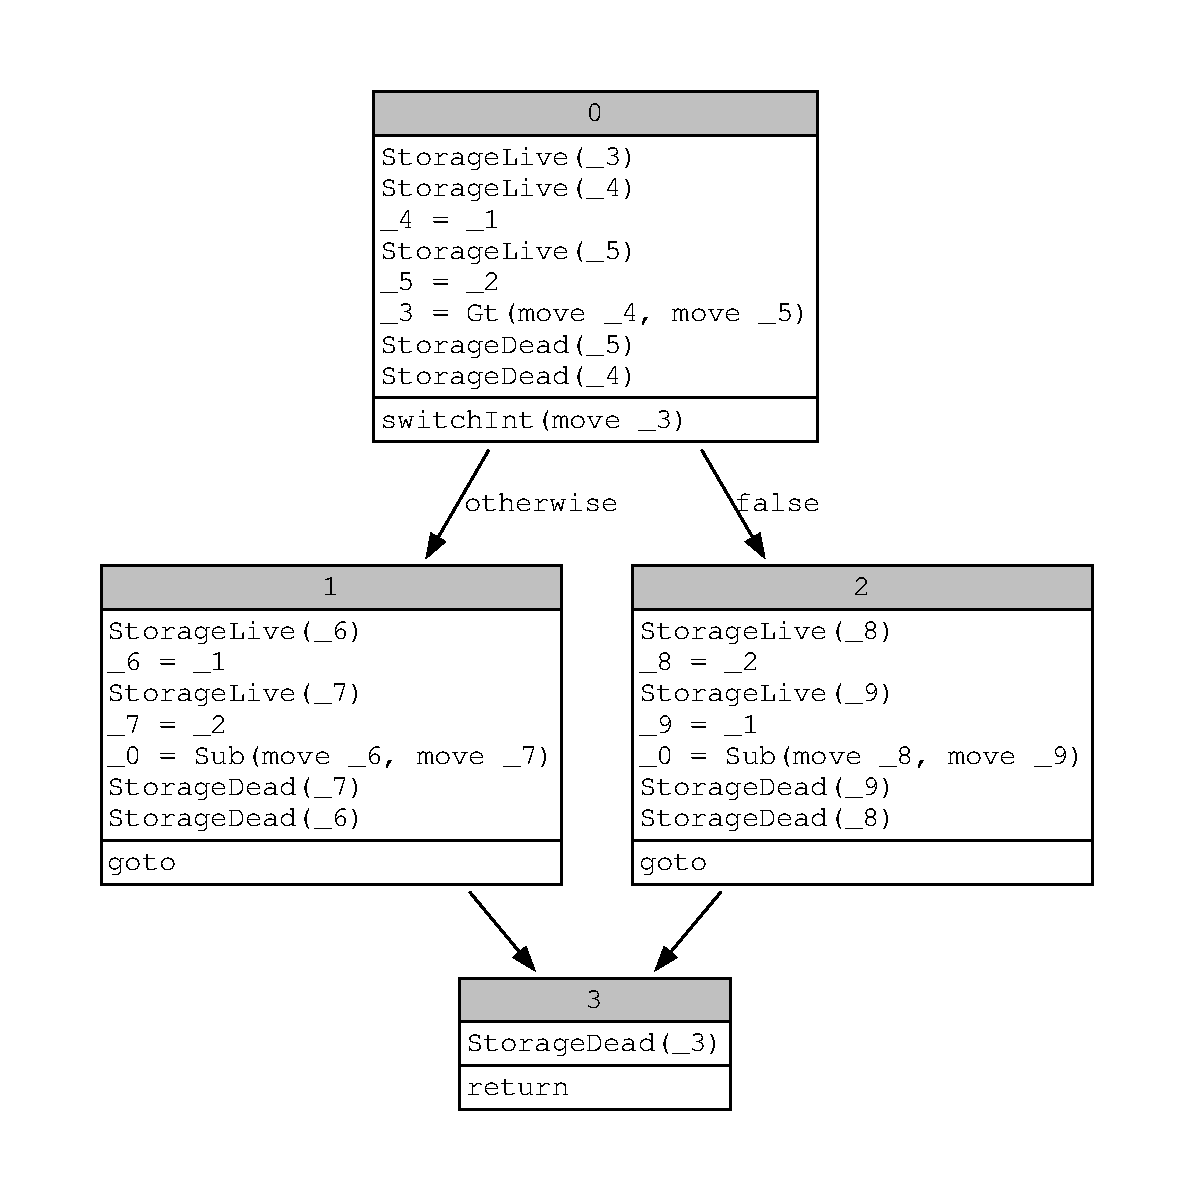
\includegraphics[height=12cm]{images/distance.pdf}
    \caption{The \textsc{mir} of the \inrust{distance} function on \fref{lst:rust_sire_example}}
  \label{lst:mir_sire_example}
\end{figure}

\begin{listing}[h]
    \begin{minted}{lisp}
    (defun distance (int 32) (int 32) (int 32) 
        (switch (> _1 _2) 
            ((const bool 0) -> (- _2 _1)) 
             (else -> (- _1 _2))))
    \end{minted}
    \caption{The \textsc{sir} of the \inrust{distance} function on \fref{lst:rust_sire_example}}
  \label{lst:sir_sire_example}
\end{listing}

\begin{listing}[h]
    \begin{minted}{lisp}
    (define-fun distance 
     ((x1 (_ BitVec 32)) (x2 (_ BitVec 32))) (_ BitVec 32) 
     (ite (bvsgt x1 x2) (bvsub x1 x2) (bvsub x2 x1)))
    \end{minted}
    \caption{The \textsc{smt-lib} snippet for the \textsc{sir} of the \inrust{distance} function on \fref{lst:rust_sire_example}}
  \label{lst:smt_sire_example}
\end{listing}


\subsection{Equality of symbolic functions}

Two \textsc{sir} functions are considered equal if they have the same type and
evaluate to the same expression for every possible argument. For simple
arithmetic expressions, this could be achieved via E-unification. However,
\textsc{sir} functions contain control flow operations and recursive calls, in
this case a theorem prover such as Z3 is up to the task. \textsc{sire} can
transform every \textsc{sir} function into an small snippet in the
\textsc{smt-lib} format to use it in an SMT solver.

Integer types on \textsc{sir} are transformed into \textsc{smt-lib} bit vectors
of the corresponding length and the signed or unsigned arithmetic operations
are transformed according to the type of the operands. Switch expressions are
transformed into nested conditionals, preserving the order of the switch
expression's branches. An example of such snippets can be found on
\fref{lst:smt_sire_example}. 

To decide if two functions are equal, is enough to write an small
\textsc{smt-lib} snippet checking if the two functions are equal in their whole
range. On \fref{lst:func_equality}, the \inrust{distance} function is compared
with an alternative implementation found on \fref{lst:alt_distance}. 

\begin{listing}[h]
    \begin{minted}{rust}
    fn alt_dist(x: i32, y: i32) -> i32 {
        let sign: i32; 
        if x > y {
           sign = 1;
        } else {
           sign = -1;
        }
        sign * (x - y)
    }
    \end{minted}
    \caption{An alternative implementation of the \inrust{distance} function on \fref{lst:rust_sire_example}}
  \label{lst:alt_distance}
\end{listing}

\begin{listing}[h]
    \begin{minted}{lisp}
    ;; Definition of distance provided by sire
    (define-fun distance 
     ((x1 (_ BitVec 32)) (x2 (_ BitVec 32))) (_ BitVec 32) 
     (ite (bvsgt x1 x2) (bvsub x1 x2) (bvsub x2 x1)))

    ;; Definition of alt_dist provided by sire
    (define-fun alt_dist 
     ((x1 (_ BitVec 32)) (x2 (_ BitVec 32))) (_ BitVec 32) 
     (ite (bvsgt x1 x2) 
      (bvmul (_ bv1 32) (bvsub x1 x2)) 
      (bvmul (_ bv4294967295 32) (bvsub x1 x2))))
    
    ;; Assert that the functions are equal
    (assert (forall ((x1 (_ BitVec 32)) (x2 (_ BitVec 32))) 
     (= (distance x1 x2) (alt_dist x1 x2)))) 

    ;; Check if the assertions can be satisfied
    (check-sat) ; sat
    \end{minted}
    \caption{equality check between the \inrust{distance} and \inrust{alt_dist} functions}
  \label{lst:func_equality}
\end{listing}

It is important to consider that the SMT solver might find no answer to one of
this queries. As a consequence, is not possible to do typechecking or type
inference for every program with generics over constant values.

\section{Typechecking of generics over constants}

\section{Generic traits over constants}

The RFC-2000 allows the user to write implementations for traits which are
generic over constant values, solving the problem of implementing traits for
arrays of arbitrary size as shown in \fref{lst:trait_const_generics}. However,
there is no mechanism to extend trait specialization for generics over constant
values. As a consequence, if a trait has several implementations for a single
type as in \fref{lst:trait_const_generics_spec} is necessary to decide which
implementation will be used on each case. 

\begin{listing}[h]
	\begin{minted}{rust}
    impl<A: Sized, B, const N: usize> PartialEq<[B; N]> 
    for [A; N] where A: PartialEq<B> {
        fn eq(&self, other: &[B; N]) -> bool {
            self[..] == other[..]
        }
        fn ne(&self, other: &[B; N]) -> bool {
            self[..] != other[..]
        }
    }
	\end{minted}
    \caption{Implementing the \inrust{PartialEq} trait for all array sizes}
  \label{lst:trait_const_generics}
\end{listing}

\begin{listing}[h]
	\begin{minted}{rust}
    impl<const N: usize> PartialEq<[i32; N]> for [i32; N]
    with {N + 1 > 1} {
        ...
    }
   
    impl<const N: usize> PartialEq<[i32; N]> for [i32; N]
    with {N > 0} {
        ...
    }
	\end{minted}
    \caption{Two implementations of a trait for the same type}
  \label{lst:trait_const_generics_spec}
\end{listing}

The basic strategy to decide which implementation to use is based on the notion
of specificity: If there is more than one implementation of a trait for the
same type, the compiler will give priority to the one which is more specific.
\footnote{More information about trait specialization can be found at
\href{https://github.com/rust-lang/rfcs/blob/master/text/1210-impl-specialization.md}{RFC-1210}.}

When generics are taken into account, this means that an implementation with
boundless generics is less specific that one with bounded generics. At the same
time, an implementation with bounded generics is more specific than one without
bounds. Finally, when two implementations have bounded generics, the
specificity degree will be decided by the specificity of its bounds. One bound
is more specific than another if the first implies the second.

Naturally, an SMT solver is capable of checking if one predicate implies
another, meaning that we can take the \textsc{sir} of the bounds and decide if
one is more specific than another. To decide which implementation is more
specific in \fref{lst:trait_const_generics_spec}, is enough to generate an
\textsc{smt-lib} snippet like the one found in \fref{lst:trait_spec_smt}.

When the SMT solver is not able to decide which bound is more specific, the
same posture as in RFC-1210 can be taken and throw an error telling the user
that the implementations are overlapping.

\begin{listing}[h]
	\begin{minted}{lisp}
        ;; Definition of bound_a provided by sire
        (define-fun bound_a
         ((x1 (_ BitVec 64))) Bool 
         (bvugt (bvadd x1 (_ bv1 64)) (_ bv1 64)))

        ;; Definition of bound_b provided by sire
        (define-fun bound_b 
         ((x1 (_ BitVec 64))) Bool 
         (bvugt x1 (_ bv0 64)))

        ;; Assert that the first bound implies the second
        (assert (forall ((x1 (_ BitVec 64))) 
         (implies (bound_a x1) (bound_b x1))))

        ;; Check if the assertions can be satisfied
        (check-sat) ; sat
	\end{minted}
    \caption{Checking if \inrust{N + 1 > 1} is more specific than \inrust{N > 0}.}
  \label{lst:trait_spec_smt}
\end{listing}

\section{Bounds for generics over constants}

\begin{listing}[h]
	\begin{minted}{rust}
    fn head<T, const N: usize>(array: &[T; N]) -> &T
    where {N > 0} {
        &array[0]
    }
    \end{minted}
    \caption{Type-safe access to the first element of an array without using
    \inrust{Option<T>}}
  \label{lst:head_const_generics}
\end{listing}

% !TEX root = ../main.tex
\chapter{Conclusion and Future work}
\label{chap:conclusion}

\section{Conclusion}

The objective of this thesis was to provide Rust with generics over constants
as a means to facilitate the language's capabilities to write generic code over
constants.

In this regard, it is certain that adding constant expressions as a kind of
parameter over generic types has improved the expressiveness and ergonomy of
Rust when dealing with constant abstraction. In particular, these additions
make the array types first class entities of the language, allowing to
implement traits over all its sizes and providing a safe mechanism to
manipulate them with static guarantees. These changes also allow for a more
natural definition of user defined types which have information that will not
change during execution and thus can be encoded in constant values as generic
parameters.

It is expected that following this design would allow for a more performant
execution of functions dealing with statically verifiable conditions. However,
It is important to remark that this design would increase compilation time
given the complexity of verifying if a set of statements is satisfiable.

Some prospects of future work are given in the rest of this chapter.


\section{Future work}

Even though \textsc{sire} is able to interpret a subset of the Rust's
\textsc{mir}, it is important to extend the coverage of \textsc{mir}
expressions. In particular, we consider of utmost importance adding support for
loops, panicking functions and algebraic data types:

\begin{itemize}

    \item Loops are the most common way of writing repetitive tasks in Rust
        even though recursion is supported. Given that loops are represented in
        \textsc{mir} as blocks with their terminators looping between them,
        this would require promoting loops to functions to transform it to a
        recursive representation suitable for the \textsc{smt-lib} format.         

    \item One of the biggest concerns of using any kind of generics is allowing
        programs with generic types that would produce unexpected behaviour after
        monomorphization. Checking on which cases a function panics, would allow
        the compiler to avoid monomorphization of generic types on those cases, or
        to at least warn the user about them.

    \item On the other hand, algebraic data types are needed to implement
        interesting structures such as bounded integers to improve the ergonomy
        of type safe access of arrays and to allow the usage of constants with
        types \inrust{Option<T>} and \inrust{Result<T, E>} as type parameters.
        To fully support algebraic data types, it is necessary to support
        \textsc{mir} projections to represent field access in structures.

\end{itemize}

Even though using an SMT solver makes our solution simpler in terms of
implementation, it adds an additional dependency if these changes were to be
added to the compiler. It is also true that an SMT solver is far from the
notion of zero-cost abstraction, because it would be more performant to write a
logic system to deal only with Rust's characteristics. Thus, we consider
necessary to provide an alternative verification mechanism, one option would be
to extend the chalk\footnote{\url{https://github.com/rust-lang/chalk}} project
to deal with these verifications.

As a final prospect, integrating this project with the compiler codebase would
simplify maintenance of the new features exposed on this work. This codebase
would fit under the constant evaluation modules of the compilers code, given
its closeness to \textsc{miri}.


% \part*{Appendix}
% \addcontentsline{toc}{part}{Appendix}
% \appendix %---------------------------------------
% \input{chapters/appendix}


 \clearemptydoublepage

 \printglossaries

 \addcontentsline{toc}{chapter}{Bibliography}
 \bibliography{bibliography/literature}

\end{document}
